% Layout/TeX-File nach Vorlage von Michael Stapelberg
% http://code.stapelberg.de/git/bewegliche-ebene/tree/poster/poster.tex


\documentclass[a0,portrait]{a0poster}

\usepackage[ngerman]{babel}
\usepackage{multicol, fontspec, amsmath, fancybox, listings, nonfloat, color, soul}

\textwidth785mm
\parindent0mm
\oddsidemargin-13pt
\evensidemargin-13pt
\renewcommand\baselinestretch{1.35}
\setlength{\fboxrule}{3.25mm}
\setlength{\fboxsep}{5mm}
\setlength{\columnsep}{30mm}
\setlength{\columnseprule}{1pt}
\linethickness{0.1mm}

\definecolor{darkyellow}{rgb}{.85,.85,0}
\definecolor{darkblue}{rgb}{0,0,.6}
\definecolor{darkred}{rgb}{.6,0,0}
\definecolor{darkgreen}{rgb}{0,.6,0}
\definecolor{darkgray}{gray}{.3}
\definecolor{lightblue}{rgb}{0.97,0.99,1}


\lstdefinestyle{colors}{keywordstyle={\bf\color{darkblue}}, commentstyle={\em\color{magenta}}, stringstyle={\color{darkred}},emphstyle={\color{darkgray}}}
\lstset{language=python, frame=single, style=colors}
\lstnewenvironment{code}{%
	\lstset{frame=single, language=python, basicstyle=\footnotesize\ttfamily, style=colors, moreemph={fabsf, sgn}}
}{}

\newenvironment{figurehere}
  {\def\@captype{figure}}
      {}
      \makeatother


\begin{document}

\begin{center}
	\vspace*{35mm}
	{\fontsize{120}{148} \textbf{Webcamsteuerung mit Raspberry Pi}\\}
	\vspace*{35mm}
	{\Large \textbf{Philip Bell}}, B.Sc. Mathematik, 7. Semester - 
	{\Large \textbf{Johannes Visintini}}, B.Sc. Angewandte Informatik, 7. Semester\\
	\vspace*{5mm}
	{\Large \textbf{Betreut durch:} Markus Kurz bzw. Gero Plettenberg und Thomas Kloepfer}
	\vspace*{15mm}
\end{center}

\begin{picture}(0,0)
	\put(20.0, 80){
\includegraphics[height=60mm]{iwr_logo/IWR-Logo-2cm-600.png}}
\end{picture}

\Ovalbox{\parbox{\textwidth}{
\begin{multicols}{2}

	\textbf{Vorwort:}\\
	Dies ist eine Kurz-Präsentation unseres Praktikums. Für ausführlichere
	Informationen besuchen Sie bitte die Praktikumshomepage [1]. Uns erreichen
	Sie unter den folgenden E-Mail Adressen:

	\begin{itemize}
		\item philip.bell@web.de
		\item visintini@stud.uni-heidelberg.de
	\end{itemize}

	\textbf{Aufgabenstellung:}\\
	Bau eines Gerüstes inkl. Schwenkvorrichtung für die Kamera und Erstellung
	eines Webservers mit folgenden Funktionen:

	\begin{itemize}
		\item Anzeige eines Live-Streams
		\item UI zur Steuerung der Kamera
	\end{itemize}

\end{multicols}
}}

\vspace*{0.01\textheight}

\Ovalbox{\begin{minipage}{\textwidth}
\begin{multicols}{2}
	
	\textbf{Haltevorrichtung:}\\
	Der Zweck dieses Teils ist einerseits alle anderen Segmente der
	Konstruktion zusammenzuhalten; andererseits sollte er die Montage an einer
	Wand erlauben. Zudem sollte die Haltevorrichtung über einen stabilen
	Stand verfügen. Wir entschieden uns zu der für diese Zwecke funktionalen
	T-Form.

	\textbf{Schwenkvorrichtung:}\\
	Dieser Teil der Konstruktion ermöglicht die Ausrichtung der Kamera. Diese
	Funktionalität wird durch zwei Servomotoren unterstützt, von denen jeweils
	einer zur horizontalen und einer zur vertikalen Orientierung verwendet
	wird.

	\textbf{Hardware:}\\
	Wir haben die folgende Hardware benutzt:\\

	\vbox{\begin{itemize}
		\item Raspberry Pi Model B Revision 2
		\item Raspberry Pi Camera Board
		\item Standard Analog Servo MC-410
	\end{itemize}}
		
	\begin{figurehere}
		\centering
		\includegraphics[height=450px,angle=90]{haltevorrichtung.jpg}\hspace{5em}
		\includegraphics[height=450px,angle=90]{schwenkvorrichtung.jpg}
	\end{figurehere}



\end{multicols}
\end{minipage}}

\vspace*{0.01\textheight}

\Ovalbox{\begin{minipage}{\textwidth}
\begin{multicols}{2}
	
	\textbf{Webserver:}\\
	Das Frontend ist mehrstufig aufgebaut. Der mJPG-Streamer mit Plugin für die
	raspicam des Raspberry Pi stellt den Stream in einer selbst gebauten
	HTML-Seite dar. Dieser wird als Dienst beim booten gestartet und läuft
	(unabhängig von den anderen Komponenten des Setups).\\


	\textbf{jQuery:}\\
	Die Webcam kann auf verschiedene Arten in horizontaler und vertikaler
	Richtung gedreht werden.

	Es gibt drei Möglichkeiten:\\
	Die \textit{triviale}:  Buttons\\
	Die \textit{intuitive}: Pfeiltasten\\
	Die \textit{mobile}:    Wischen\\

	Alle drei Möglichkeiten werden von Funktionen unter Zuhilfenahme der
	JavaScript-Bibliothek jQuery abgefangen. Im Hintergrund werden dann über
	diese Funktionen Anfragen an den Server gestellt, unter Übermittlung der
	gewünschten Bewegungsrichtung.

	Die mobile Variante von jQuery sorgt gleichzeitig für ein schöneres
	(Grund-)Design der Webseite.\\


	\textbf{Apache:}\\
	Als Webserver wird Apache verwendet, der als sehr stabil gilt. Dieser
	fungiert als Instanz, die mit dem Browser des Clients kommuniziert.
	Sämtlicher Datenverkehr (auch zum mJPG-Streamer) läuft über Apache. Der
	Webserver nimmt auch die Steuerbefehle entgegen und leitet sie über ein
	WSGI-Skript, das eine Verbindung zum moveserver aufbaut, an denselben
	weiter. Dieses WSGI-Skript überprüft auch, ob die Bewegungsrichtung erlaubt
	ist. So können falsche Werte nicht an den moveserver weitergegeben werden.\\\vspace{7.5em}


	\textbf{Sicherheit:}\\
	Da der Raspberry Pi als ganz normaler Computer bzw. Server im öffentlichen
	Netz hängt, musste sich überlegt werden wie dieser gegenüber Angriffe aus
	dem Internet abgesichert wird.

	Als Firewall wird die populäre Firewall *iptables* und zur einfacheren
	Konfiguriation derselben *firehol* verwendet. Diese ist so konfiguriert,
	dass nur Anfragen aus dem Universitätsnetz, das als sicher gilt, akzeptiert
	werden. Außerdem sind nur die Dienste *http* (Port 80, für den Webserver)
	und *ssh* (Port 22, zur Konfiguriation und Wartung) freigegeben.

	Durch ständige Updates und die oben erwähnte Firewall wird gewährleistet,
	dass der Raspberry Pi im Internet mindestens so geschützt ist, wie die
	meisten anderen Server.\\
		
	\begin{figurehere}
		\centering
		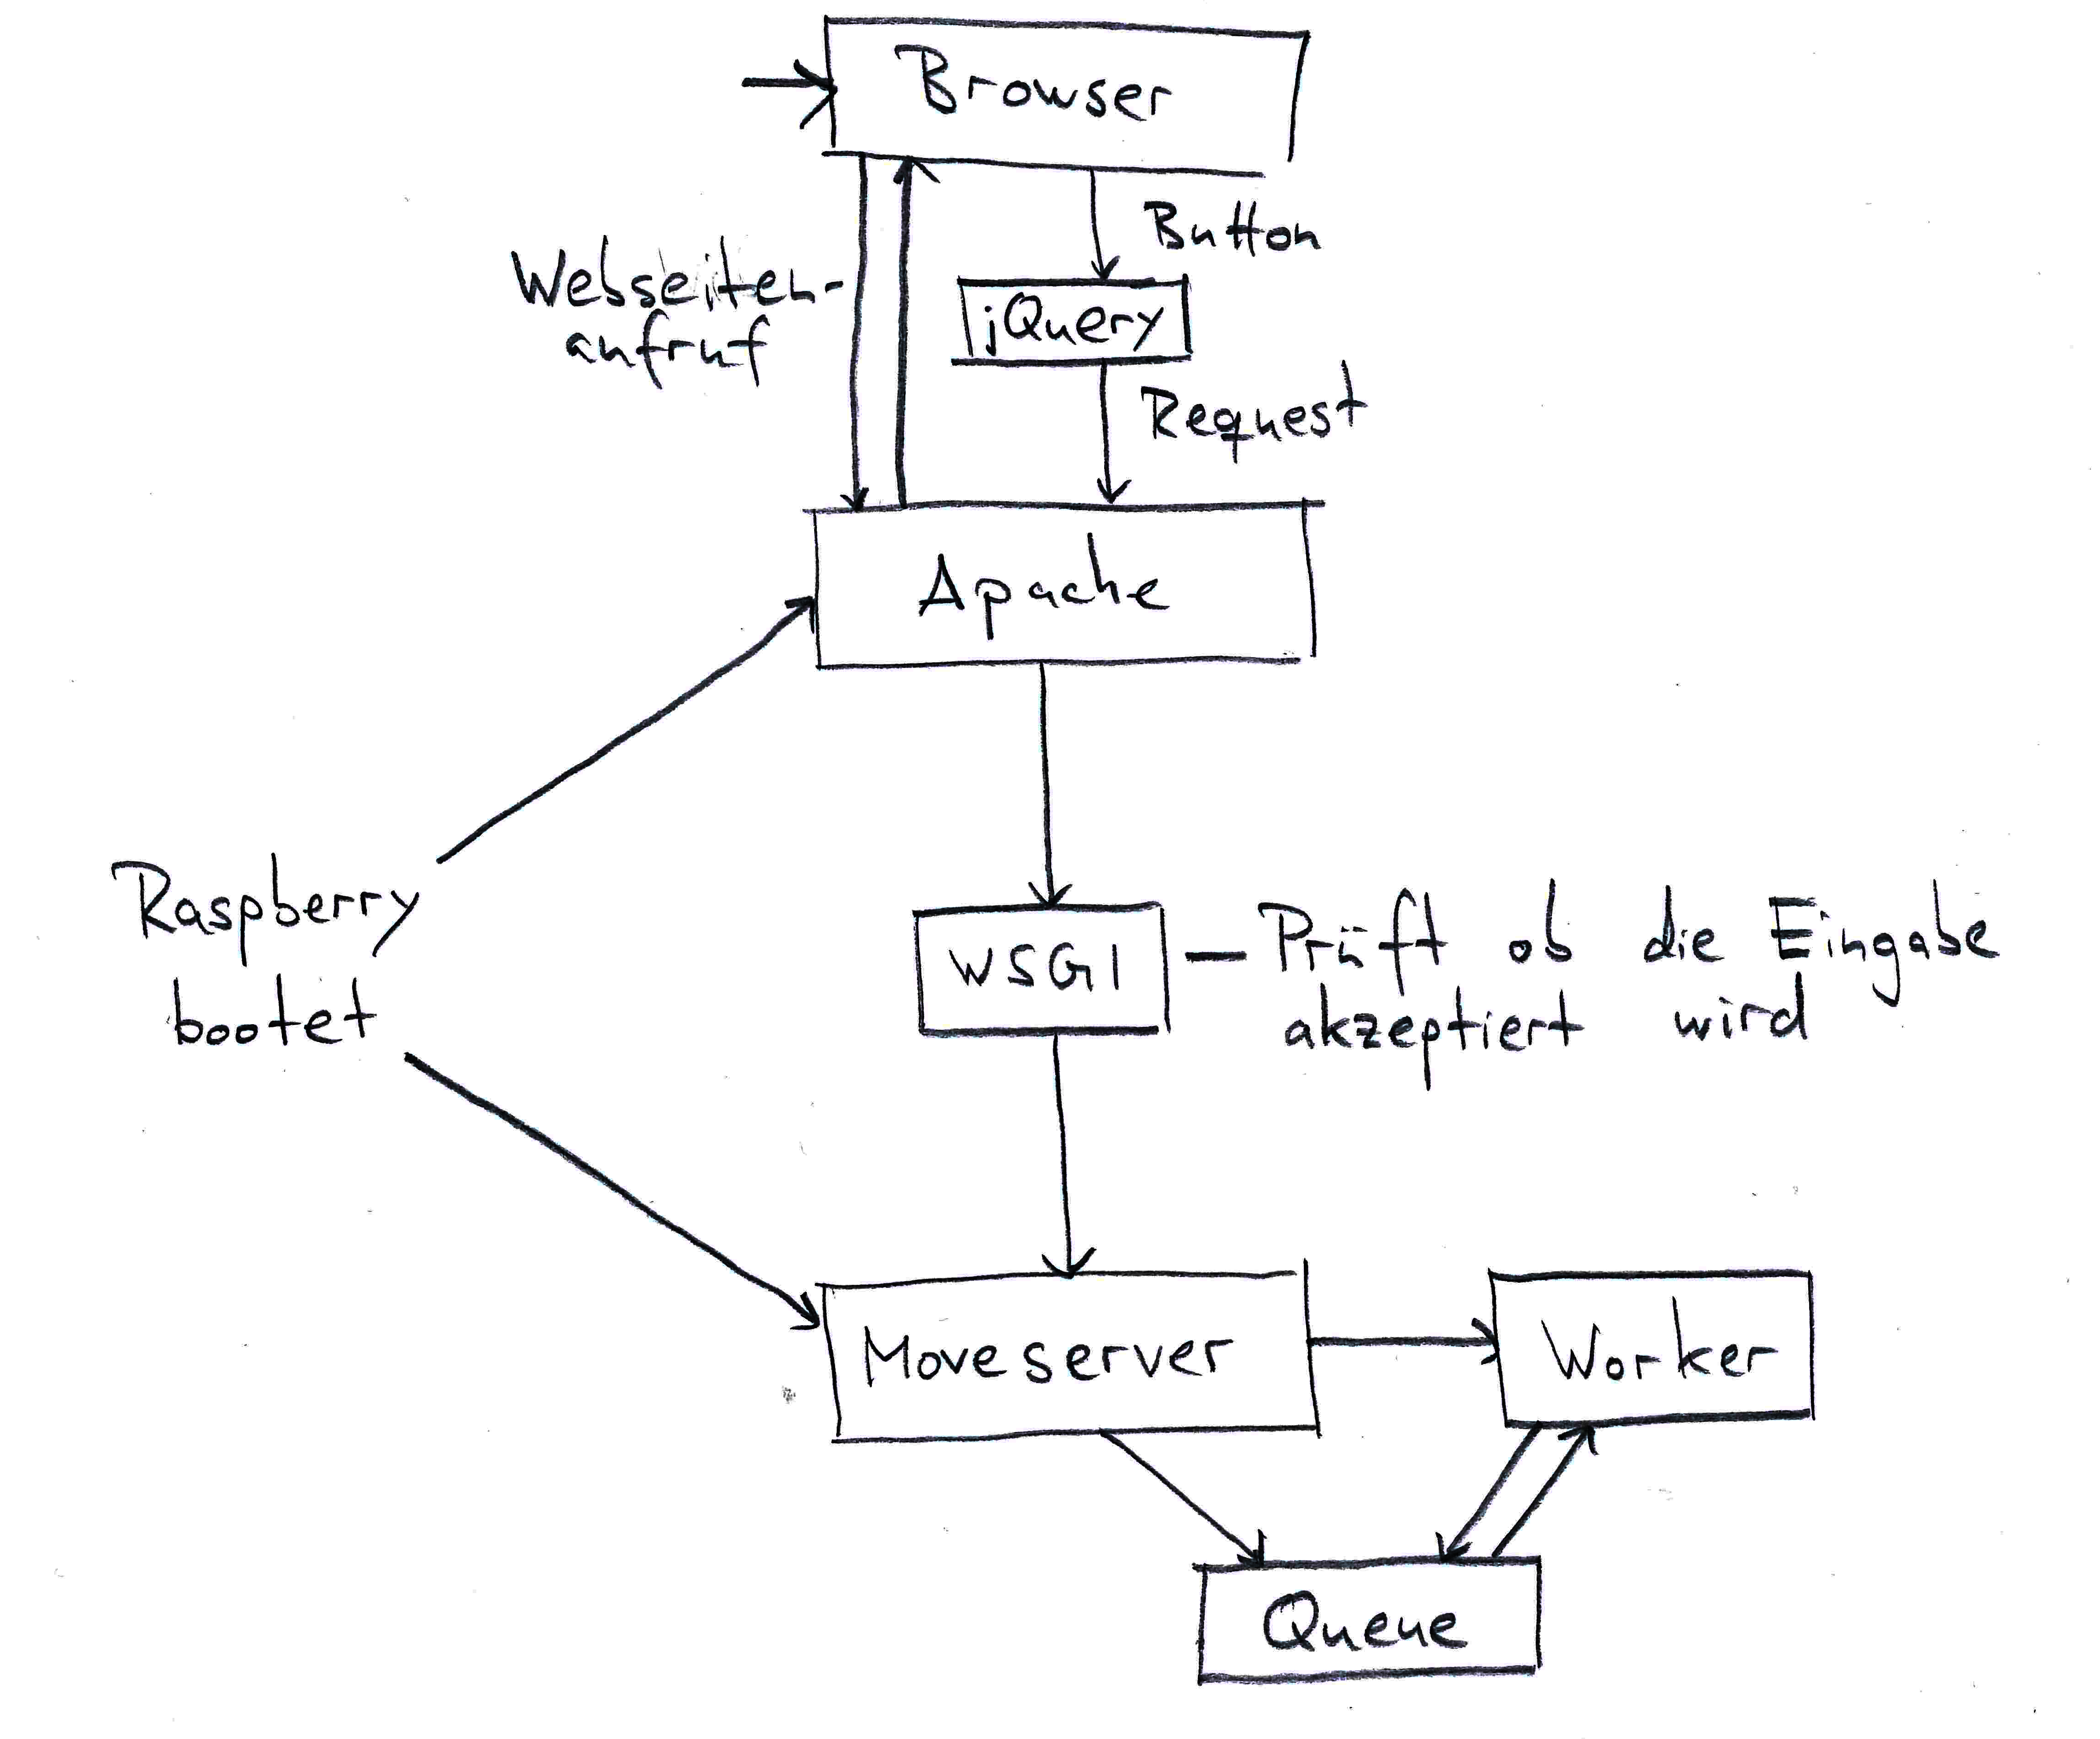
\includegraphics[width=.24\textwidth]{kontrollflussdiagramm.png}
		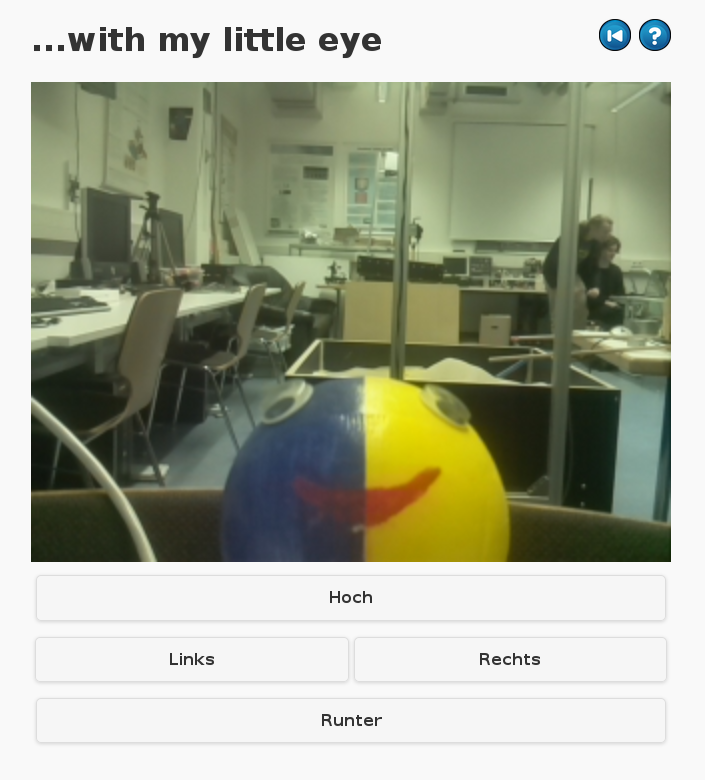
\includegraphics[width=.24\textwidth]{websitescreenshot.png}
	\end{figurehere}


\end{multicols}
\end{minipage}}

\vspace*{0.01\textheight}

\Ovalbox{\begin{minipage}{\textwidth}
\begin{multicols}{2}

	\textbf{moveserver:}\\
	Der moveserver ist ein Pythonskript, das beim Einschalten des Raspberry
	gestartet wird. Zuerst einmal stellt er sicher, dass die Servos zu Beginn
	in eine bekannte Stellung, die wir als die Standardposition bezeichnen,
	gebracht werden, da ein Auslesen der Position aus den Servos nicht möglich
	ist. Weiterhin füllt er die vom WSGI-Skript erhaltenen Requests in die
	Queue und startet den Worker (s.u.). Zusätzlich führt er die
	Suspend-Funktionalität als Subprozess aus und verwaltet deren
	Zeit-Variable.\\


	\textbf{Queue \& Worker:}\\
	Die eingehenden Requests werden in einer Queue (LIFO) der Länge 5
	zwischengespeichert, dh die zuerst eingehenden Requests werden zuerst vom
	Worker abgearbeitet. Ist die Queue voll, wird der älteste Befehle
	verworfen. Diese Form der Priorisierung hat sich als funktional erwiesen:
	Auch in einer Testsituation, in der ein Testskript massiv viele Requests
	sendete, konnte ein Mensch die Steuerung, wenngleich nur mit intensivem
	Einsatz, beeinflussen. Hier folgt ein Auszug, der vom Worker aufgerufene
	Funktion \textit{move()}:

	(den gesamten Code gibt es auf http://github.com/joker234.de/fp\_webcam)\\

	\begin{code}
	  # tmp: position to move, step: Schrittweite
	  # nr:  Number of the GPIO-pin. 4 = vertical move, 17 = horizontal move.
	  if direction == "left":
	    print "move %s" % direction;
	  # Festlegen welcher Servo bewegt wird
	    nr = 4;
	  # Überprüfen ob der maximale Ausrichtungswinkel nicht überschritten wird
	  # Die Zahl gibt dabei die Signallänge, mit der die Servos angesprochen
	  # werden, in Mikrosekunden an
	  # Wir lassen eine Signallänge von 1000 bis 2000 zu; die lässt etwa eine
	  # Drehung um 90 Grad in beide Richtungen von der Mittelstellung (1500) zu
	    if curr4 + step <= 2000:
	      curr4 += step;
	    else:
	      curr4 = 2000;
	    tmp = curr4;
	  # Drehen des entsprechenden Servo (nr) zum angegebenen Ausrichtungswinkel (tmp)
	  go_servo(nr, tmp);
	\end{code}


\end{multicols}
\end{minipage}}


\end{document}
